\documentclass[20pt,a0paper,blockverticalspace=7mm]{tikzposter}

\usepackage[american]{babel}
\usepackage[utf8]{inputenc}
\usepackage[T1]{fontenc}
\usepackage{amsmath,amssymb}
\usepackage{url}
\usepackage{wrapfig,graphicx}
\usepackage{array}
\usepackage{algorithmic}
\renewcommand{\algorithmicrequire}{\textbf{Input:}}
\renewcommand{\algorithmicensure}{\textbf{Output:}}
\algsetup{linenodelimiter=.}
\usepackage{colortbl}
\usepackage[export]{adjustbox}
\usepackage{tikz}
\usetikzlibrary{matrix,arrows,arrows.meta,positioning}
\tikzset{>/.tip={Computer Modern Rightarrow[scale=2,line width=1pt]}}
\tikzset{|/.tip={Bar[scale=2,line width=1pt]}}
\tikzset{c_/.tip={Hooks[scale=2,line width=1pt,right]}}
\tikzset{c^/.tip={Hooks[scale=2,line width=1pt,left]}}

\def\Q {\ensuremath{\mathbb{Q}}}
\def\Z {\ensuremath{\mathbb{Z}}}
\def\F {\ensuremath{\mathbb{F}}}
\def\Tr {\ensuremath{\mathrm{Tr}}}
\def\M {\ensuremath{\mathsf{M}}}
\def\tildO {\ensuremath{\mathrm{\tilde{O}}}}

\DeclareMathOperator{\Gal}{Gal}
\DeclareMathOperator{\ord}{ord}

\renewcommand{\paragraph}[1]{\smallskip\textbf{#1}}
\newcommand{\secblock}[1]{\block[]{}{\huge\sc #1}}

\title{Computing isomorphisms and embeddings of finite fields}
\author{Ludovic Brieulle\footnotemark[1], Luca De Feo\footnotemark[2],
  Javad Doliskani\footnotemark[3], Jean-Pierre Flori\footnotemark[4],
  Éric Schost\footnotemark[3]}
\institute{\footnotemark[1]Université d'Aix-Marseille,
  \footnotemark[2]Université de Versailles -- Saint-Quentin-en-Yvelines,\\
  \footnotemark[3]University of Waterloo,
  \footnotemark[4]Agence Nationale de Sécurité des Systèmes d'Information}

\usetheme{Desert}

\definecolorpalette{UVSQ}{
    \definecolor{colorOne}{RGB}{255,255,255}
    \definecolor{colorTwo}{RGB}{0,146,187}
    %\definecolor{colorThree}{RGB}{119,173,28}
}
\colorlet{alert}{red}
\usecolorstyle[colorPalette=UVSQ]{Sweden}

\definetitlestyle{WLogos}{
    width=\paperwidth, roundedcorners=0, linewidth=0pt, innersep=1.5cm,
    titletotopverticalspace=0mm, titletoblockverticalspace=7mm,
    titlegraphictotitledistance=10pt, titletextscale=1
}{
   \draw[draw=none, bottom color=titlebgcolor, top color=framecolor,opacity=0.9]%
   (\titleposleft,\titleposbottom) rectangle (\titleposright,\titlepostop); %
   \draw
   (\titleposleft+2em,0.75*\titlepostop+0.25*\titleposbottom)
   node[anchor=west]{\includegraphics[width=15em]{amu}}
   (\titleposright-1em,0.75\titlepostop+0.25*\titleposbottom)
   node[anchor=east]{\includegraphics[width=15em]{uvsq-logo-cmjn}}
   (\titleposleft,\titleposbottom+4.5em)
   node[anchor=west]{\includegraphics[width=20em]{uwaterloo}}
   (\titleposright-5em,\titleposbottom+1.5em)
   node[anchor=south east]{\includegraphics[height=6em]{Anssi}};
}
\usetitlestyle{WLogos}

\pgfmathsetseed{\number\pdfrandomseed} 
\definebackgroundstyle{FancyBack}{
  \draw[opacity=0.2] (0,0) 
  node[rotate={random(0,359)}]{\includegraphics[height=\textheight]{Anssi}};
}
\usebackgroundstyle{FancyBack}

\begin{document}
\maketitle

\begin{columns}
  %%%%%%%%%%%%%%%%%
  % Intro
  %%%%%%%%%%%%%%%%%
  \column{0.333}

  \block{The embedding problem}{
    \begin{wrapfigure}{r}{0.45\colwidth}
      \hfill
      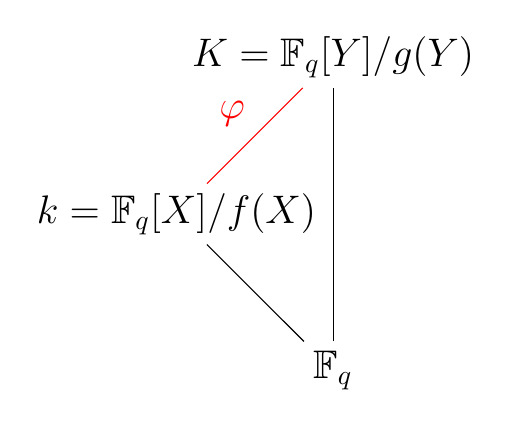
\begin{tikzpicture}[node distance=8em,font=\Large]
        \node(Fq){$\F_q$};
        \node(Fqf)[above left of=Fq]{$k=\F_q[X]/f(X)$};
        \node(Fqg)[above right of=Fqf]{$K=\F_q[Y]/g(Y)$};
        \draw[]
        (Fq) edge (Fqf)
        (Fq) edge (Fqg)
        (Fqf) edge[left,auto,color=alert] node{$\varphi$} (Fqg);
      \end{tikzpicture}
    \end{wrapfigure}

    \paragraph{Let}
    \begin{itemize}
    \item $\F_q$ be a field with $q$ elements,
    \item $f$ and $g$ be irreducible polynomials in $\F_q[X]$ and
      $\F_q[Y]$,
    \item $m=\deg f$, $n=\deg g$ and $m|n$.
    \end{itemize}

    There exists a field
    embedding \[\color{alert}\varphi:k\hookrightarrow K,\] unique up to
    \mbox{$\F_q$-auto}morphisms of $k$.

    \paragraph{Goals}
    \begin{itemize}
    \item \textbf{Represent} $\varphi$ efficiently,
    \item \textbf{Evaluate/Invert} $\varphi$ efficiently,
    \end{itemize}

    When $\deg f = \deg g$, this is also called the
    \emph{isomorphism problem}. 
    
    \paragraph{Applications}
    \begin{itemize}
    \item Fundamental building blocks of computer algebra systems.
    \item Work algorithmically in the algebraic closure
      $\bar{\F}_q$~\cite{bosma+cannon+steel97}.
    \end{itemize}
  }

  \block{Embedding description}{ 
    \begin{wrapfigure}[6]{r}{0.4\colwidth}
      \centering
      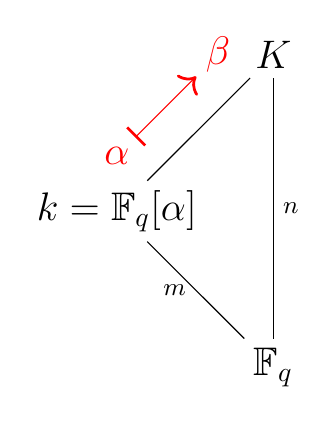
\begin{tikzpicture}[node distance=8em,font=\Large]
        \node(Fq){$\F_q$};
        \node(Fqf)[above left of=Fq]{$k=\F_q[\alpha]$};
        \node(Fqg)[above right of=Fqf]{$K$};
        \begin{scope}[alert,node distance=2em]
          \node(a)[above of=Fqf]{$\alpha$};
          \node(b)[left of=Fqg]{$\beta$};
        \end{scope}
        \draw[auto,font=\small]
        (Fq) edge node[left]{$m$} (Fqf)
        (Fq) edge node[right]{$n$} (Fqg)
        (Fqf) edge (Fqg);
        \draw[|->,alert]
        (a) edge (b);
      \end{tikzpicture}
    \end{wrapfigure}

    \textbf{Determine} elements $\alpha\in k$ and $\beta\in K$ such
    that

    \begin{itemize}
    \item $\alpha$ generates $k=\F_q[\alpha]$,
    \item there exists $\varphi:\alpha\mapsto\beta$.
    \end{itemize}

    \paragraph{Naive solution:} take
    \begin{itemize}
    \item $\alpha= X \mod f(X)$, and
    \item $\beta$ a root of $f$ in $K$.
    \end{itemize}
    Cost of factorization: $\tildO(mn^{(\omega+1)/2})$
  }

  \block{Embedding evaluation}{ 
    \begin{wrapfigure}[8]{r}{0.2\colwidth}
      \centering
      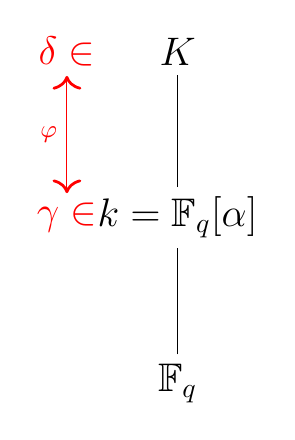
\begin{tikzpicture}[node distance=6em,font=\Large,on grid]
        \node(Fq){$\F_q$};
        \node(Fqf)[above=of Fq]{$k=\F_q[\alpha]$};
        \node(Fqg)[above=of Fqf]{$K$};
        \begin{scope}[alert,node distance=4em]
          \node(a)[left=of Fqf]{$\gamma\in$};
          \node(b)[left=of Fqg]{$\delta\in$};
        \end{scope}
        \draw
        (Fq) edge (Fqf)
        (Fqf) edge (Fqg);
        \draw[<->,alert]
        (a) edge node[left,auto,font=\small]{$\varphi$} (b);
      \end{tikzpicture}
    \end{wrapfigure}

    \textbf{Given}
    \begin{itemize}
    \item a \emph{description} of the embedding (as above),
    \item $\gamma\in k$ and $\delta\in K$,
    \end{itemize}

    \textbf{Solve} the following problems:
    \begin{itemize}
    \item Compute $\varphi(\gamma)$ in $K$.
    \item Test if $\delta\in\varphi(k)$.
    \item Supposing $\delta\in\varphi(k)$, compute $\varphi^{-1}(\delta)$ in $k$.
    \end{itemize}
    
    \textbf{Naive solution:} Linear algebra (size $n\times m$).

    \textbf{Better solutions:} Not presented here. See~\cite{ffisom-long}.
  }

  \block{History of embedding description}{
    \begin{description}
    \item['91] Lenstra~\cite{LenstraJr91} proves that the isomorphism
      problem is in $\mathsf{P}$.
      \begin{itemize}
      \item Based on Kummer theory, pervasive use of linear algebra.
      \item Does not prove precise complexity. Rough estimate:
        $\Omega(n^3)$.
      \end{itemize}
    \item['92] Pinch's algorithm~\cite{Pinch}:
      \begin{itemize}
      \item Based on mapping algebraic groups over $k,K$.
      \item Incomplete algorithm, no complexity analysis.
      \end{itemize}
    \item['96] Rains~\cite{rains2008} generalizes Pinch's algorithm.
      \begin{itemize}
      \item Complete algorithm, rigorous complexity analysis.
      \item Unpublished. Leaves open question of using elliptic
        curves.
      \end{itemize}
    \item['02] Allombert's variant of Lenstra's algorithm~\cite{Allombert02,Allombert02-rev}:
      \begin{itemize}
      \item Trades determinism for efficiency.
      \item Implementation integrated into Pari/GP.
      \end{itemize}
    \item['07] Magma implements Rains' algorithm.
    \item['16] Narayanan proves the first $\tildO(n^2)$ upper
      bound~\cite{narayanan2016fast}.
      \begin{itemize}
      \item Variant of Allombert's algorithm.
      \item Using asymptotically fast modular composition.
      \end{itemize}
    \item[This work:] knowledge systematization. Notable results:
      \begin{itemize}
      \item Better variants of Allombert's algorithm.
      \item $\tildO(n^2)$ upper bound \emph{without fast modular
          composition}.
      \item Generalized Rains' algorithm to elliptic curves.
      \item C/Flint/Sage implementations, experiments, comparisons.
      \end{itemize}
    \end{description}
  }

  \column{0.333}
  
  \block{Allombert's algorithm}{
    For simplicity, we reduce to $m=n$ a prime power.
    
    \begin{wrapfigure}[8]{r}{0.35\colwidth}
      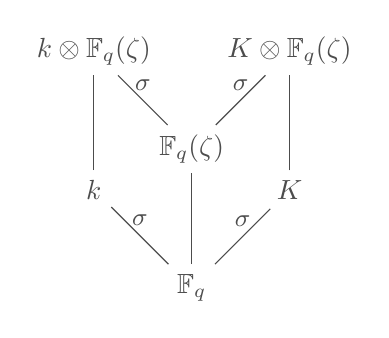
\begin{tikzpicture}[node distance=5em,on grid,black!70]
        \node(Fq){$\F_q$};
        \node(Fqz)[above=of Fq]{$\F_q(\zeta)$};
        \node(k)[above left=of Fq]{$k$};
        \node(kz)[above=of k]{$k\otimes\F_q(\zeta)$};
        \node(K)[above right=of Fq]{$K$};
        \node(Kz)[above=of K]{$K\otimes\F_q(\zeta)$};
        \draw[font=\small,above]
        (Fq) edge (Fqz)
        (Fq) edge node{$\sigma$} (k)
        (Fqz) edge node{$\sigma$} (kz)
        (k) edge (kz)
        (Fq) edge node{$\sigma$} (K)
        (Fqz) edge node{$\sigma$} (Kz)
        (K) edge (Kz);
      \end{tikzpicture}
    \end{wrapfigure}

    \paragraph{Technique (assuming $\gcd(n,q)=1$)}
  
    \begin{itemize}
    \item Let $h$ be an irreducible factor of the $n$-th cyclotomic
      polynomial over $\F_q$;
    \item Extend the action of $\Gal(k/\F_q)$ to the \textbf{ring}
      $k[\zeta]=k[Z]/h(Z)$:
      \[\begin{array}{llll}
          \sigma: & k[\zeta] & \rightarrow & k[\zeta], \\
                  & x \otimes \zeta & \mapsto & \sigma(x) \otimes \zeta;
        \end{array}\]
    \end{itemize}
    
    \begin{itemize}
    \item \textbf{Solve Hilbert 90:} find $\theta_1 \in k[\zeta]$ such that
      $\sigma(\theta_1) = \zeta\theta_1$;
    \item Compute $\theta_2 \in K[\zeta]$ similarly;
    \item Find $c\in\F_q(\zeta)$ such that $c=\theta_1 / \theta_2$;
    \item Project $\theta_1\mapsto\alpha\in k$ and
      $c\theta_2\mapsto\beta\in K$.
    \end{itemize}

    Similar algorithm for the Artin-Schreier case $\gcd(n,q)\ne 1$.
  }

  \block{Solving Hilbert 90}{
    We look for an element in the kernel of $\sigma-\zeta$.
    \begin{description}
    \item[Allombert] Use linear algebra.
      \hfill\textcolor{blue}{$\tildO(n^3)$}
      or \textcolor{blue}{$\tildO(n^{\omega+1/2})$}      
    \item[Classic trick (already in Lenstra)] Use the equality
      \[\sigma^n-1 = (\sigma-\zeta)\circ\Theta(\sigma) =
        (\sigma-\zeta)\circ\sum_{i=0}^{r-1}\zeta^{-i-1}\sigma^i,\]
      evaluate $\Theta(\sigma)$ on random element of $k[\zeta]$.
    \end{description}

    We give three \textbf{new} strategies, complexity depends on
    $s\equiv\ord\sigma$:

    \medskip

    \begin{tabular}{>{\bfseries}l p{0.45\colwidth}
      @{\hspace{5ex}}>{\color{black!70}}p{0.32\colwidth}}
      \arrayrulecolor{black!30}\hline
      1. & Evaluate $\Theta(\sigma)$ by divide-and-conquer, using
           modular composition.
      & Similar to Narayanan, good for small $s$.\\
      \hline
      2. &  Let $(S^n-1)=h(S)\cdot g(S)$, then
           \[\sigma^n-1 = h(\sigma)\circ g(\sigma).\]
           Evaluate $g(\sigma)$ via \emph{automorphism evaluation}~\cite{kaltofen+shoup98},
           then $h(\sigma)/(\sigma-\zeta)$.
      & Best practical performance\\
      \hline
      3. & Evaluate $\Theta(\sigma)$ directly via \emph{iterated
           frobenius}~\cite{vzgathen+shoup92}.
      & Best complexity: \textcolor{blue}{$\tildO(n^2)$}
    \end{tabular}
  }

  \block{Rain's algorithm}{
    \begin{wrapfigure}[1]{r}{0pt}
      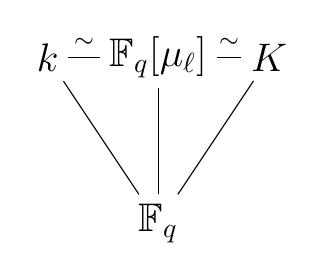
\begin{tikzpicture}[node distance=6em,font=\Large,on grid]
        \node(Fq){$\F_q$};
        \node(kum)[above=of Fq]{$\F_q[\mu_\ell]$};
        \node(k)[left=4em of kum]{$k$};
        \node(K)[right=4em of kum]{$K$};
        \draw[auto,font=\small]
        (Fq) edge (kum)
        (Fq) edge (k)
        (Fq) edge (K)
        (k) edge node{$\sim$} (kum)
        (kum) edge node{$\sim$} (K);
      \end{tikzpicture}
    \end{wrapfigure}

    \paragraph{Pinch's idea}
    \begin{itemize}
    \item Find \emph{small} $\ell$ such that $k\simeq\F_q[\mu_\ell]$,
    \item Pick $\ell$-th roots of unity $\alpha\in k$, $\beta\in K$,
    \item Find $e$ s.t. $\alpha\mapsto\beta^e$.
    \item \textbf{Problem 1:} worst case $\ell\in O(q^n)$.
    \item \textbf{Problem 2:} potentially $O(\ell)$ exponents $e$ to test.
    \end{itemize}
    
    \begin{wrapfigure}[6]{r}{0.45\colwidth}
      \hfill
      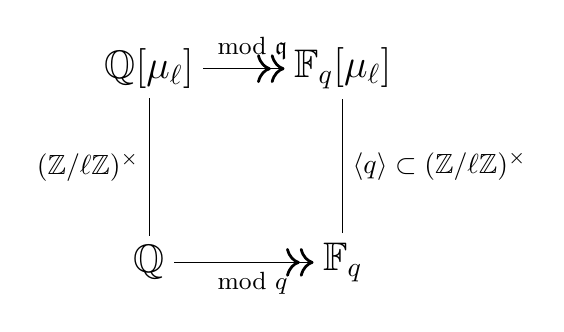
\begin{tikzpicture}[node distance=7em,font=\Large,on grid]
        \node(Fq){$\F_q$};
        \node(Q)[left=of Fq]{$\Q$};
        \node(k)[above=of Fq]{$\F_q[\mu_\ell]$};
        \node(C)[above=of Q]{$\Q[\mu_\ell]$};
        \draw[auto,font=\normalsize]
        (Fq) edge node[right]{$\langle q\rangle\subset(\Z/\ell\Z)^\times$} (k)
        (Q) edge node{$(\Z/\ell\Z)^\times$} (C);
        \draw[auto,font=\small,->>]
        (Q) edge node[below]{$\mod q$} (Fq)
        (C) edge node{$\mod\frak{q}$} (k);
      \end{tikzpicture}
    \end{wrapfigure}

    \paragraph{Rains' solution to problem 2}

    \begin{itemize}
    \item Replace $\alpha,\beta$ with \emph{Gaussian periods}:
      \[\eta(\alpha) = \sum_{\sigma\in S}\alpha^\sigma\]
      where $(\Z/\ell\Z)^\times = \langle q\rangle \times S$.
    \end{itemize}

    \begin{itemize}
    \item Periods are \emph{normal}, hence $\eta(\alpha)\mapsto\eta(\beta)$.
    \end{itemize}

    \begin{wrapfigure}[6]{r}{0.35\colwidth}
      \centering
      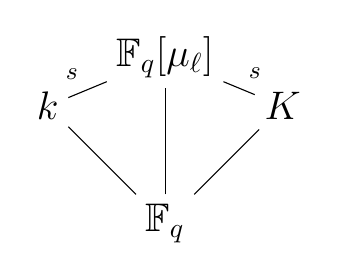
\begin{tikzpicture}[node distance=6em,font=\Large,on grid]
        \node(Fq){$\F_q$};
        \node(kum)[above=of Fq]{$\F_q[\mu_\ell]$};
        \node(k)[above left=of Fq]{$k$};
        \node(K)[above right=of Fq]{$K$};
        \draw[auto,font=\small]
        (Fq) edge (kum)
        (Fq) edge (k)
        (Fq) edge (K)
        (k) edge node{$s$} (kum)
        (kum) edge node{$s$} (K);
      \end{tikzpicture}
    \end{wrapfigure}

    \paragraph{Rains' solution to problem 1}
    \begin{itemize}
    \item Allow \emph{small} degree $s$ \emph{auxiliary}\\ extensions;
    \item Take traces to descend to $k, K$.
    \item Best bound: $\ell\in O(n^{2.4+\epsilon})$ (GRH),\\
      in practice $\ell\in O(n\log n)$.
    \end{itemize}
    
    \begin{itemize}
    \item \textbf{Practical complexity:}
      $\tildO\left(sn^{(\omega+1)/2}\right)$. Fast when $s=1$.
    \item \textbf{Limitations:}  Not really interesting for $q$ non-prime,\\
      only practical for very small $s$.
    \end{itemize}
    
    \paragraph{New elliptic variant}
    \begin{itemize}
    \item Replace $\F_q[\mu_\ell]$ with \emph{random} elliptic curves
      $E/\F_q$;
    \item Replace Gaussian periods with \emph{elliptic
        periods}~\cite{mihailescu+morain+schost07}.
    \item No need for auxiliary extension, same bounds on $\ell$:\\
      $\ell\in O(n^{2.4+\epsilon})$ (GRH),
      $\ell\in O(n\log n)$ (practical).
    \item \textbf{Practical complexity:} $\tildO\left(n^2\right)$.
    \item Note: elliptic periods \emph{are not normal}, method is
      \emph{not guaranteed to work}, but we have a:
    \end{itemize}

    \paragraph{Conjecture:} Elliptic periods generate their definition
    field.
  }

  
  \column{0.333}
  \makeatletter
  \setlength{\TP@blockverticalspace}{5mm}
  \makeatother

  \block[bodyinnersep=0]{Experimental results}{
    \begin{itemize}
    \item C/Flint implementation of Allombert's algortihm and variants,
    \item Sage/Cython implementation of Rains' and variants,
    \item Comparisons with Pari/GP, Sage, Magma ({\small $100\le q\le 2^{20}$, $3\le n\le 2069$}).
    \end{itemize}

    \newlength{\mywidth}
    \setlength{\mywidth}{0.58\colwidth}
    \begin{tabular}{p{0.35\colwidth} r}
      \raggedright
      \textbf{Allombert's algorithm,} in the case where the auxiliary degree
      $s=\ord_q(n)\le 10$.  Dots represent individual runs, lines
      represent degree 2 linear regressions.
      & \includegraphics[valign=t,width=\mywidth]{../plots/bench-allombert-lowaux} \\

      \raggedright
      \textbf{Allombert's algorithm,} as a function of the auxiliary degree
      $s=\ord_q(n)$.  Individual running times are scaled by down by
      $n^2$.  Dots represent individual runs, lines represent degree 2
      linear regressions.
      & \includegraphics[valign=t,width=\mywidth]{../plots/bench-allombert-anyaux} \\

      \raggedright
      \textbf{Rains' algorithm.} Auxiliary extension degrees $s$ for cyclotomic
      Rains' range between $1$ and $9$. Lines represent median times.
      & \includegraphics[valign=t,width=\mywidth]{../plots/bench-rains} \\
      
      \raggedright
      \textbf{Rains' algorithm.}  Our implementation vs
      Magma's. Running time of our implementation in seconds vs ratio of
      Magma running time over ours. Plot in doubly logarithmic scale.
      & \includegraphics[valign=t,width=\mywidth]{../plots/bench-magma}\\

      \raggedright
      \textbf{Allombert's vs Rains'}  at some fixed auxiliary extension
      degrees $s$. Lines represent median times, shaded areas minimum
      and maximum times.
      & \includegraphics[valign=t,width=\mywidth]{../plots/bench-all}
    \end{tabular}
      
    \begin{itemize}
    \item See the paper \url{https://arxiv.org/abs/1705.01221} for more:
      \begin{itemize}
      \item Embedding evaluation,
      \item Experimental evidence for the conjecture on elliptic periods,
      \item More algorithms and complexity analyses.
      \end{itemize}
    \item Code and data at \url{https://github.com/defeo/ffisom}.
    \end{itemize}
  }

  \block{\refname}{
    \small
    \renewcommand*{\refname}{\vspace{-1.5em}}
    \bibliographystyle{plain}
    \bibliography{../refs}
  }

\end{columns}

\end{document}